\subsection{Verification of Rates of Convergence}
In this subsection we verify the theoretical error estimates developed in
\autoref{sec:QGEError}. To this end, we apply the Argyris FE in space while
applying implicit Euler in time to \eqref{eqn:QGE_psi}. To solve the resulting
nonlinear system at each time step we apply Newton's method where the Newton's
method is considered to have converged when the $L^2$-norm of the difference in
the current Newton iterate and the previous Newton iterate is less than
$10^{-7}$. Additionally, in each of the following computational tests we take
$Re = 1$, $Ro = 1$, and $h = \nicefrac{1}{20}$ unless otherwise stated.

\subsubsection*{Test 1}
For this test we take the exact solution to be
\begin{equation}
  \psi(t;x,y) = \left(\sin \pi x \sin \pi y\right)^2 \sin t
  \label{eqn:Test1}
\end{equation}
which is very similar to \textbf{Test 6} in \cite{Foster}. Here we add the time
dependence in the sine term and let $\Omega = [0,1]^2$. The time interval for
integration is $t = [0,\frac{\pi}{2}]$. This test will have an intensifying
western boundary layer as time increases.

\begin{table}
  \begin{center}
    \begin{tabular}{|c|c|c|c|c|}
      \hline
      $k$ & $h$ & DoFs & $e_{L^2}$ & $L^2$ order \\% & $e_{H^1}$ & $H^1$ order & $e_{H^2}$ & $H^2$ order \\
      \hline
      $\nicefrac{1}{2}$ & $\nicefrac{1}{16}$ & $2853$ & $5.65\times 10^{-4}$ & $-$ \\[0.2em]%& $0.00293$ & $-$ & $0.01971$ & $-$ \\
      $\nicefrac{1}{4}$ & $\nicefrac{1}{16}$ & $2853$ & $3.49\times 10^{-4}$ & $0.697$ \\[0.2em]%& $0.001807$ & $0.6971$ & $0.01216$ & $0.697$ \\
      $\nicefrac{1}{8}$ & $\nicefrac{1}{16}$ & $2853$ & $1.916\times 10^{-4}$ & $0.864$ \\[0.2em]%& $0.0009931$ & $0.8636$ & $0.006683$ & $0.8634$ \\
      $\nicefrac{1}{16}$ & $\nicefrac{1}{16}$ & $2853$ & $1.001\times 10^{-4}$ & $0.937$ \\[0.2em]%& $0.0005189$ & $0.9366$ & $0.003494$ & $0.9359$ \\
      $\nicefrac{1}{32}$ & $\nicefrac{1}{16}$ & $2853$ & $5.11\times 10^{-5}$ & $0.970$ \\[0.2em]%& $0.000265$ & $0.9696$ & $0.001787$ & $0.9668$ \\
      $\nicefrac{1}{64}$ & $\nicefrac{1}{16}$ & $2853$ & $2.58\times 10^{-5}$ & $0.985$ \\[0.2em]%& $0.0001339$ & $0.9851$ & $0.0009098$ & $0.9743$ \\
      $\nicefrac{1}{128}$ & $\nicefrac{1}{16}$ & $2853$ & $1.30\times 10^{-5}$ & $0.993$ \\[0.2em]%& $6.728\times 10^{-5}$ & $0.9925$ & $0.0004705$ & $0.9513$ \\
      $\nicefrac{1}{256}$ & $\nicefrac{1}{16}$ & $2853$ & $6.51\times 10^{-6}$ & $0.996$ \\[0.2em]%& $3.374\times 10^{-5}$ & $0.9959$ & $0.0002607$ & $0.8516$ \\
      $\nicefrac{1}{512}$ & $\nicefrac{1}{16}$ & $2853$ & $3.26\times 10^{-6}$ & $0.998$ \\[0.2em]%& $1.691\times 10^{-5}$ & $0.9965$ & $0.0001715$ & $0.6046$ \\
      $\nicefrac{1}{1024}$ & $\nicefrac{1}{16}$ & $2853$ & $1.63\times 10^{-6}$ & $0.999$ \\[0.2em]%& $8.497\times 10^{-6}$ & $0.9927$ & $0.0001405$ & $0.2878$ \\
      \hline

    \end{tabular}
  \end{center}
  \caption{Observed order of convergence for Implicit-Euler applied to
    \eqref{eqn:QGE_psi} with the exact solution \eqref{eqn:Test1}.
    %Note the observed order of convergence matches the theoretical error estimates developed in \autoref{sec:QGEError}.
  }
  \label{tab:Test1Time}
\end{table}

\begin{figure}
  \begin{center}
    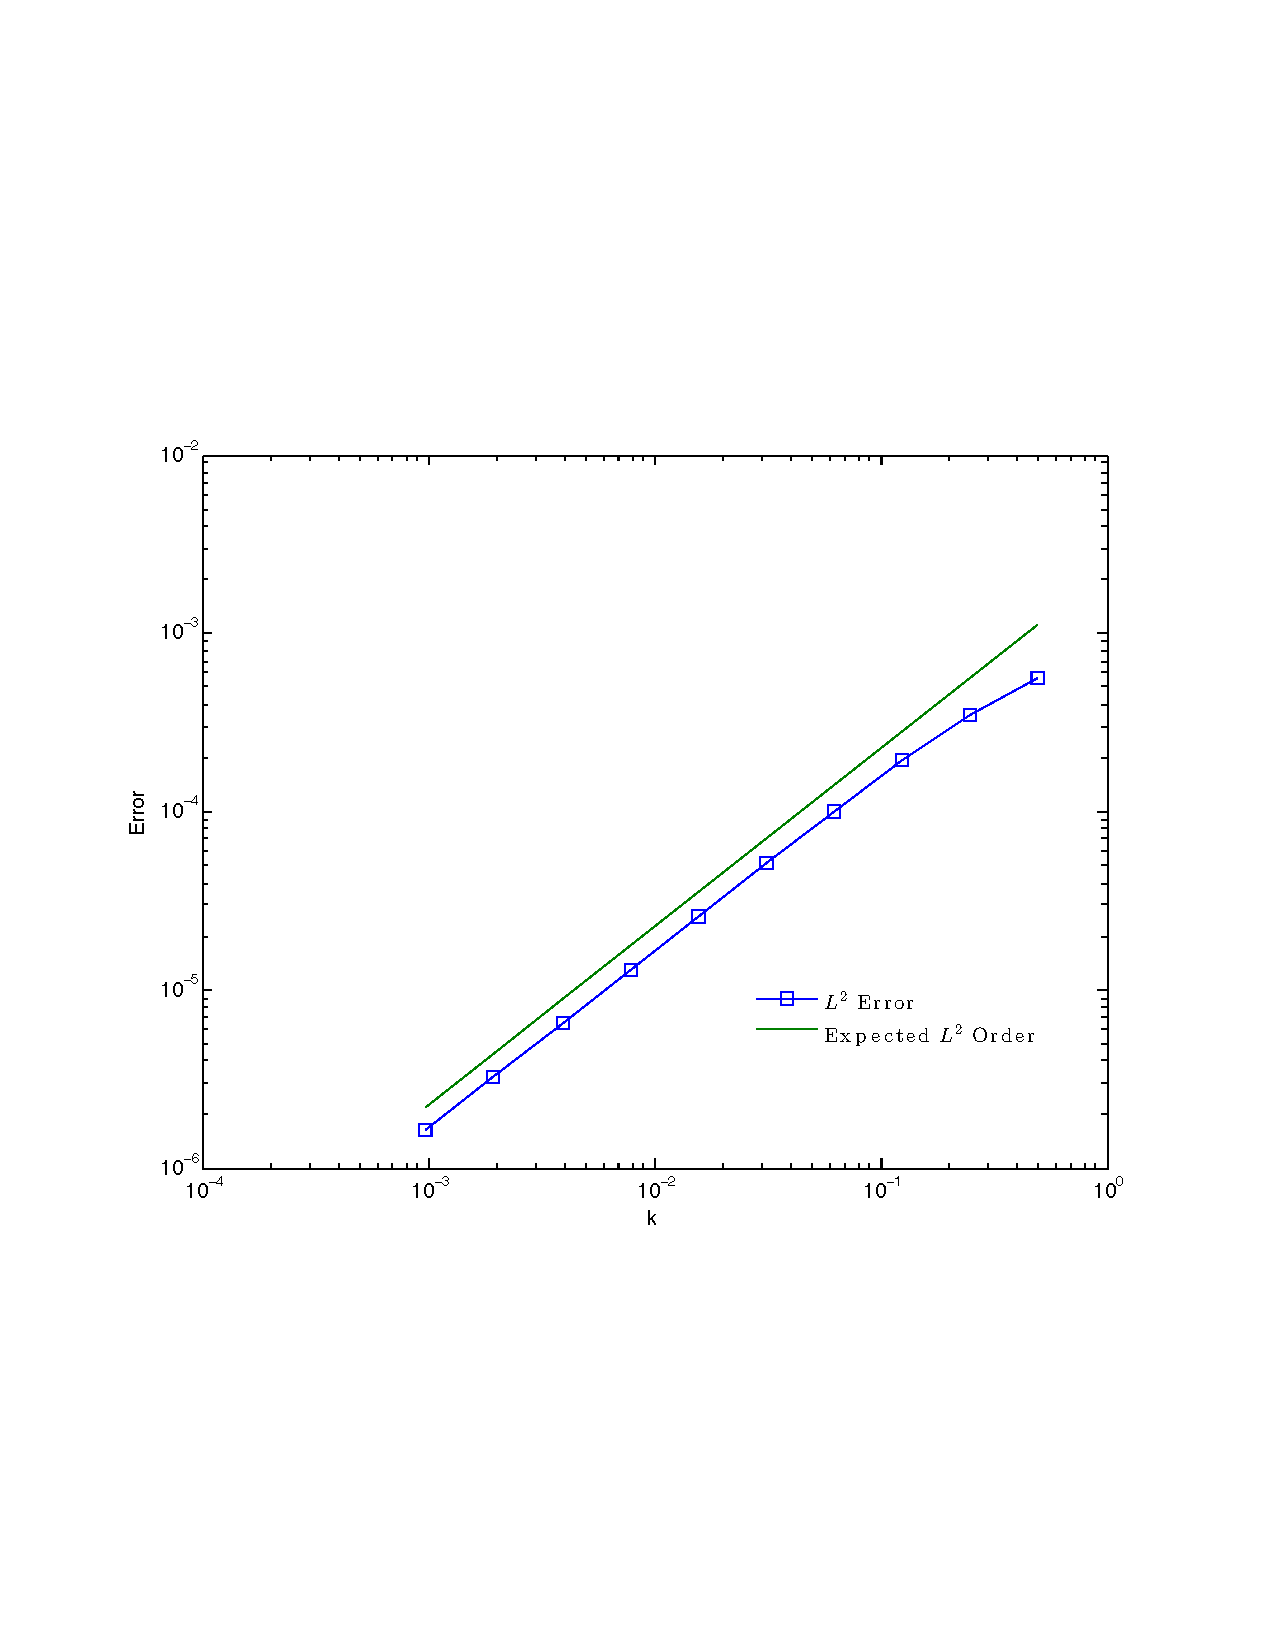
\includegraphics[scale=0.6]{Figures/sin2sin2sinTimeConvergence.pdf}
    \caption{Observed order of convergence for Implicit-Euler applied to
      \eqref{eqn:QGE_psi} with the exact solution \eqref{eqn:Test1}.}
  \label{fig:Test1Time}
  \end{center}
\end{figure}

\begin{table}
  \begin{center}
    \begin{tabular}{|c|c|c|c|c|c|c|c|c|}
      \hline
      $k$ & $h$ & DoFs & $e_{L^2}$ & $L^2$ order & $e_{H^1}$ & $H^1$ order & $e_{H^2}$ & $H^2$ order \\
      \hline
      $\nicefrac{1}{8192}$ & $\nicefrac{1}{2}$ & $38$ & $1.23\times 10^{-2}$ & $-$ & $1.18\times 10^{-1}$ & $-$ & $1.57\times 10^0$ & $-$ \\[0.2em]
      $\nicefrac{1}{8192}$ & $\nicefrac{1}{4}$ & $174$ & $2.12\times 10^{-5}$ & $9.18$ & $7.31\times 10^{-4}$ & $7.34$ & $2.79\times 10^{-2}$ & $5.81$ \\[0.2em]
      $\nicefrac{1}{8192}$ & $\nicefrac{1}{8}$ & $662$ & $7.88\times 10^{-7}$ & $4.75$ & $4.59\times 10^{-5}$ & $3.99$ & $3.04\times 10^{-3}$ & $3.20$ \\[0.2em]
      $\nicefrac{1}{8192}$ & $\nicefrac{1}{16}$ & $2853$ & $7.87\times 10^{-9}$ & $6.65$ & $9.05\times 10^{-7}$ & $5.67$ & $1.29\times 10^{-4}$ & $4.56$ \\[0.2em]
      $\nicefrac{1}{8192}$ & $\nicefrac{1}{32}$ & $11690$ & $6.97\times 10^{-11}$ & $6.82$ & $1.88\times 10^{-8}$ & $5.59$ & $5.98\times 10^{-6}$ & $4.43$ \\[0.2em]
      $\nicefrac{1}{8192}$ & $\nicefrac{1}{64}$ & $47958$ & $7.23\times 10^{-12}$ & $3.27$ & $5.26\times 10^{-10}$ & $5.16$ & $3.43\times 10^{-7}$ & $4.12$ \\[0.2em]
      \hline
    \end{tabular}
  \end{center}
  \caption{Observed spatial orders of convergence for Argyris applied to
    \eqref{eqn:QGE_psi} with the exact solution \eqref{eqn:Test1} using implicit
    Euler for time discretization. Note the observed orders of convergence
    nearly matches the theoretical error estimates developed in
    \autoref{sec:QGEError}. The $L^2$ order, however, drops off for the last
    spatial discretization due to nearing the machine epsilon.}
  \label{tab:Test1Space}
\end{table}

\begin{figure}
  \begin{center}
    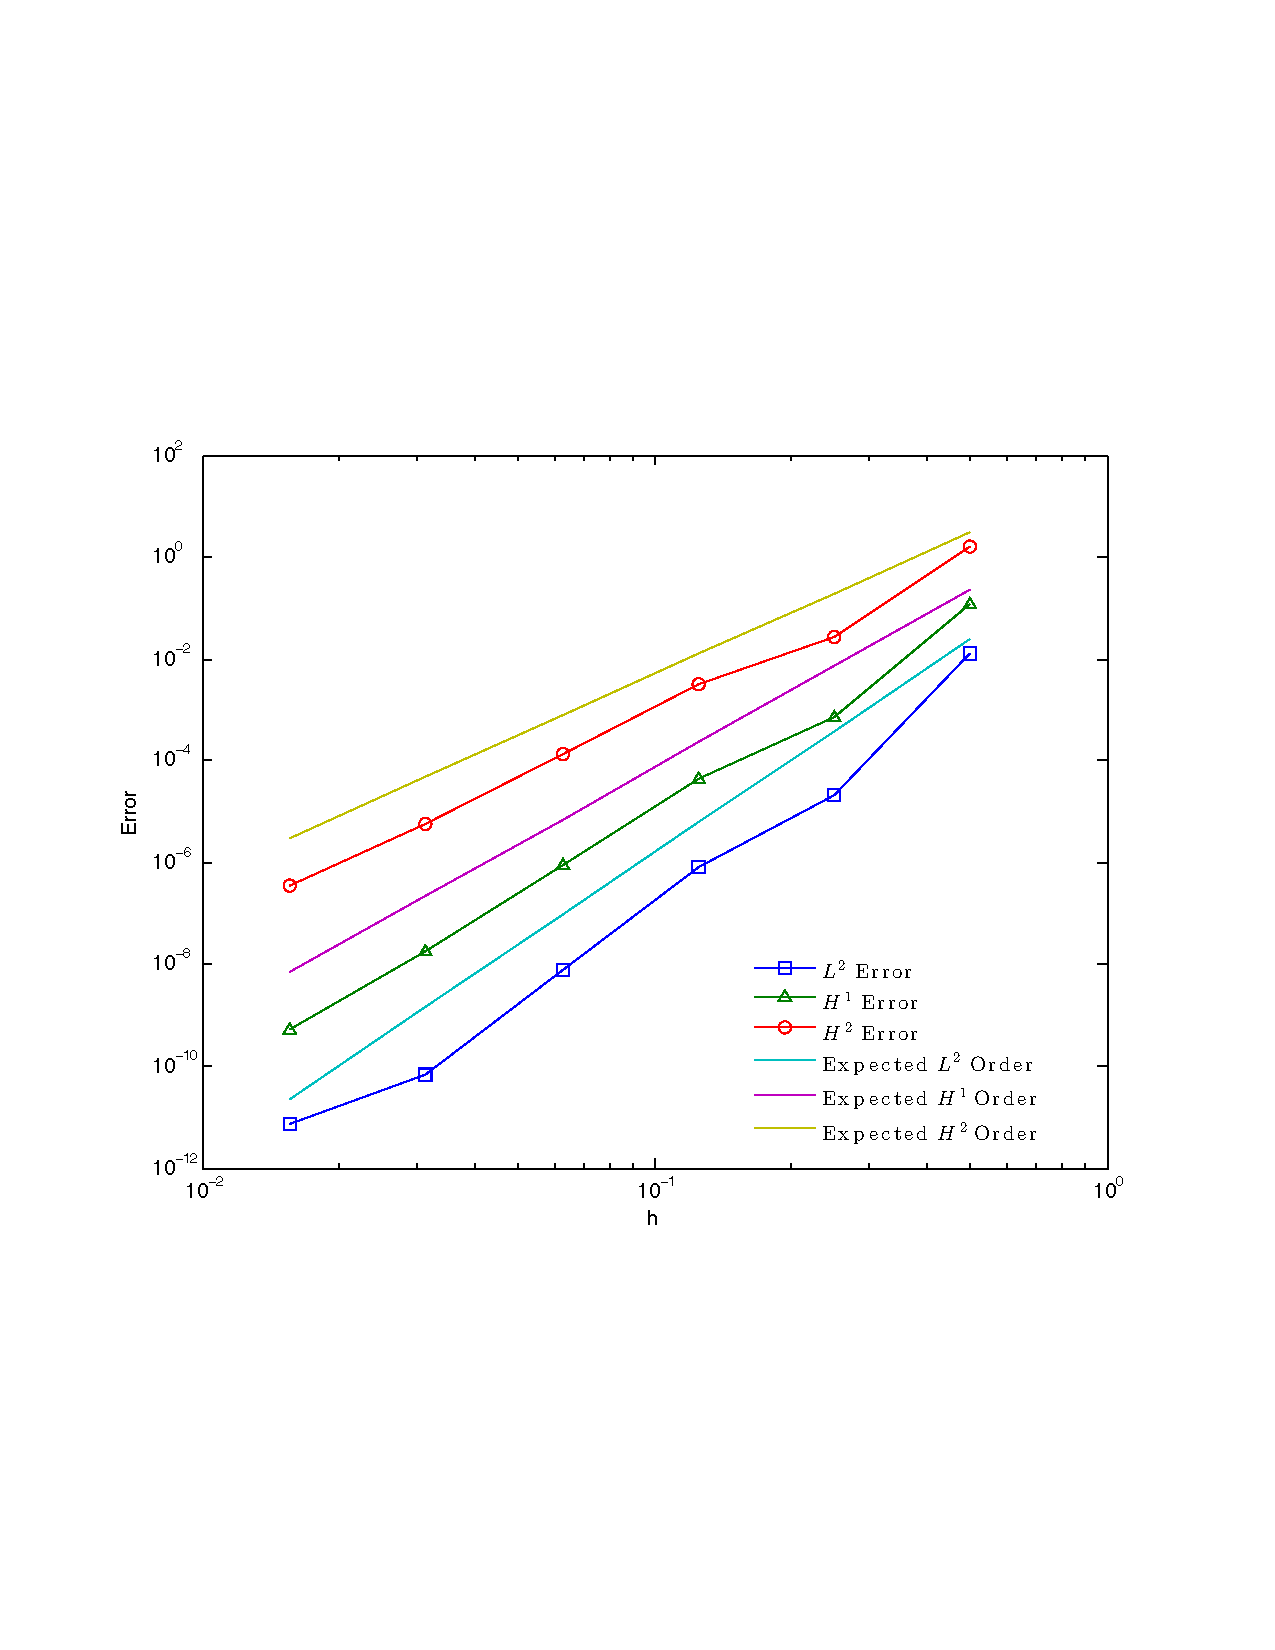
\includegraphics[scale=0.6]{Figures/sin2sin2sinSpaceConvergence.pdf}
    \caption{Observed orders of convergence in space for Argyris applied to
      \eqref{eqn:QGE_psi} with the exact solution \eqref{eqn:Test1} using
      implicit Euler for the time discretization.}
  \label{fig:Test1Space}
  \end{center}
\end{figure}

\subsubsection*{Test 2}
For this test we take the exact solution to be
\begin{equation}
  \psi(t;x,y) = \left[(1-\frac{x}{3})\left(1-e^{-20\,x}\right) \sin \pi
    y\right]^2 \sin t
  \label{eqn:Test2}
\end{equation}
which is very similar to \textbf{Test 6} in \cite{Foster}. Here we add the time
dependence in the exponential term and let $\Omega = [0,3]^2$. The time interval
for integration is $t = [0,0.5]$. This test will have an intensifying western
boundary layer as time increases.
\begin{table}
\begin{center}
  \begin{tabular}{|c|c|c|c|c|}
    \hline
    $k$ & $h$ & DoFs & $e_{L^2}$ & $L^2$ order \\
    \hline
    $\nicefrac{1}{2}$ & $\nicefrac{1}{64}$ & $47958$ & $1.52\times 10^{-4}$ & $-$\\
    $\nicefrac{1}{4}$ & $\nicefrac{1}{64}$ & $47958$ & $9.41\times 10^{-5}$ & $0.695$\\
    $\nicefrac{1}{8}$ & $\nicefrac{1}{64}$ & $47958$ & $5.17\times 10^{-5}$ & $0.865$\\
    $\nicefrac{1}{16}$ & $\nicefrac{1}{64}$ & $47958$ & $2.70\times 10^{-5}$ & $0.937$\\
    $\nicefrac{1}{32}$ & $\nicefrac{1}{64}$ & $47958$ & $1.38\times 10^{-5}$ & $0.970$\\
    $\nicefrac{1}{64}$ & $\nicefrac{1}{64}$ & $47958$ & $6.96\times 10^{-6}$ & $0.985$\\
    $\nicefrac{1}{128}$ & $\nicefrac{1}{64}$ & $47958$ & $3.50\times 10^{-6}$ & $0.993$\\
    $\nicefrac{1}{256}$ & $\nicefrac{1}{64}$ & $47958$ & $1.75\times 10^{-6}$ & $0.996$\\
    $\nicefrac{1}{512}$ & $\nicefrac{1}{64}$ & $47958$ & $8.78\times 10^{-7}$ & $0.998$\\
    $\nicefrac{1}{1024}$ & $\nicefrac{1}{64}$ & $47958$ & $4.40\times 10^{-7}$ & $0.996$\\
    \hline
  \end{tabular}
\end{center}
  \caption{Observed order of convergence for Implicit-Euler applied to
    \eqref{eqn:QGE_psi} with the exact solution \eqref{eqn:Test2}. Note the observed
    order of convergence matches the theoretical error estimates developed in
    \autoref{sec:QGEError}.}
  \label{tab:Test2Time}
\end{table}

\begin{figure}
  \begin{center}
    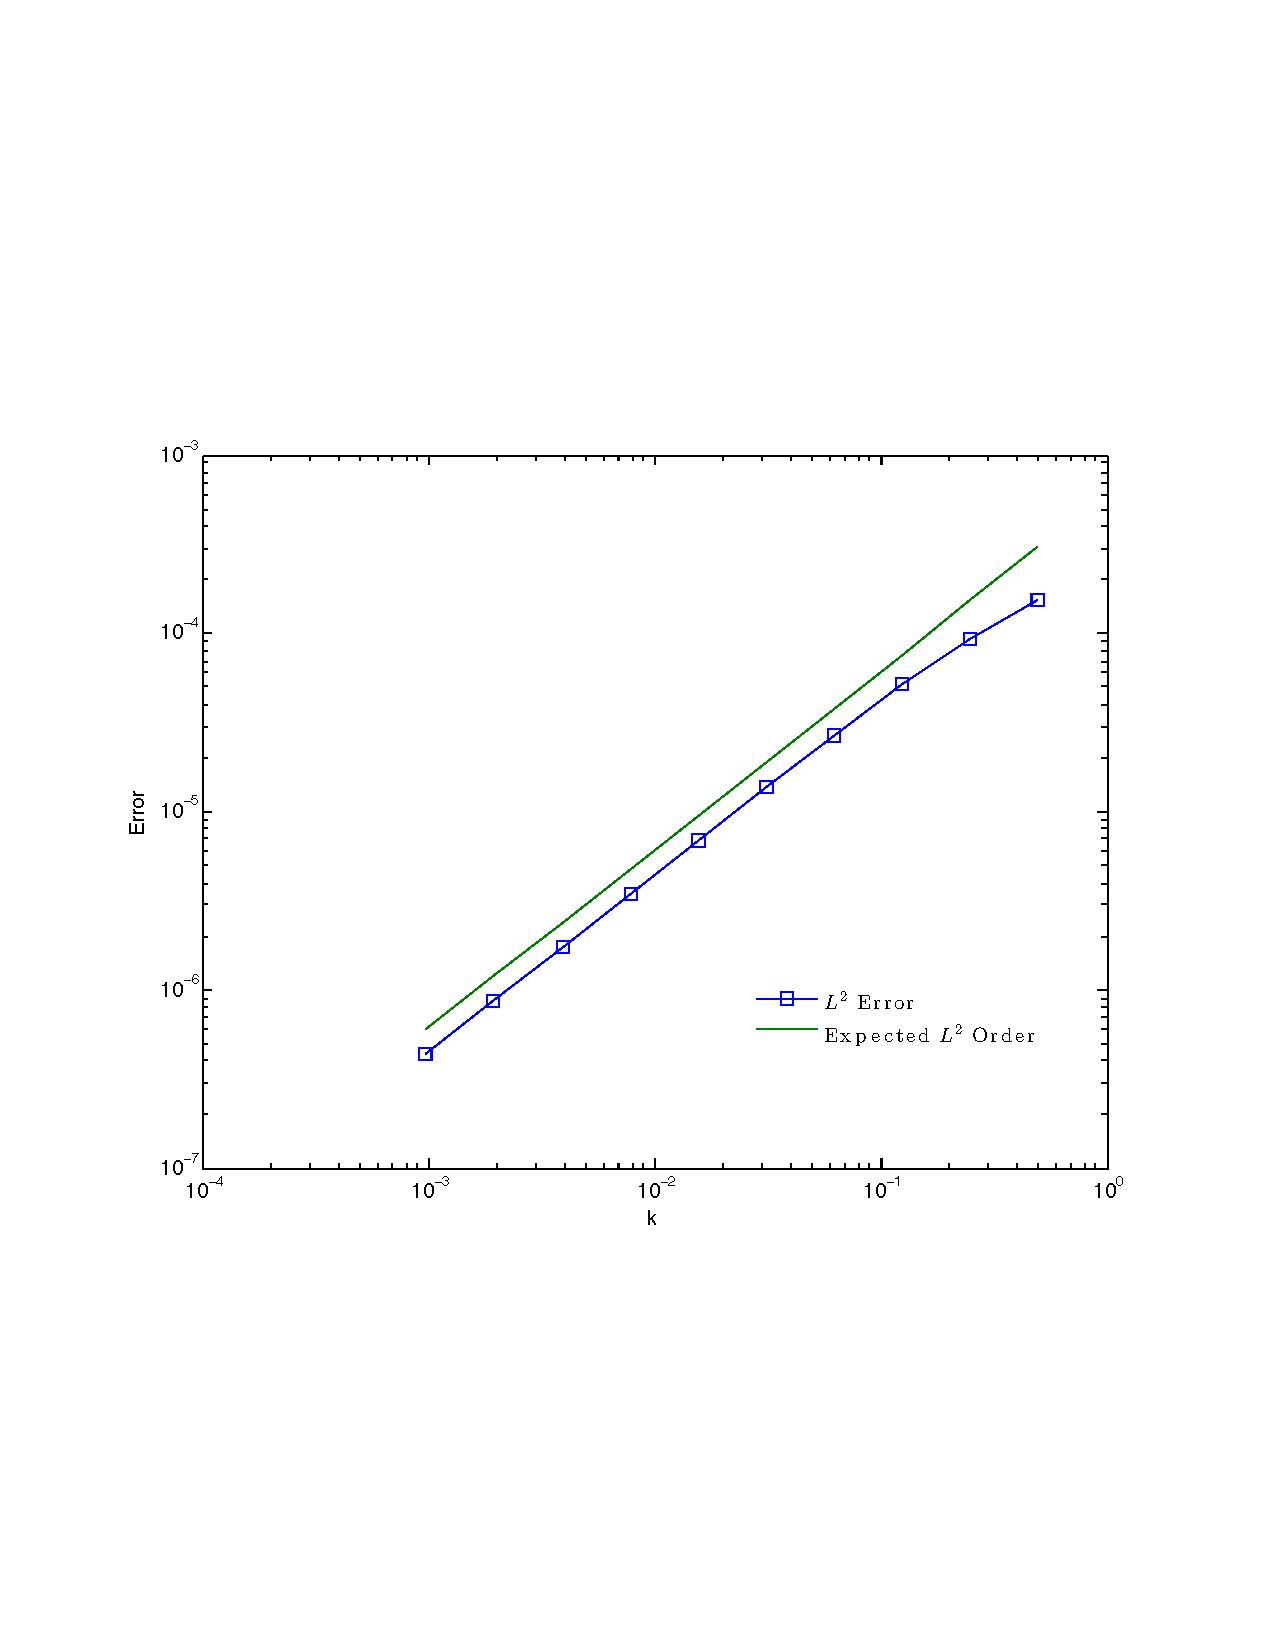
\includegraphics[scale=0.6]{Figures/expsinTimeConvergence.pdf}
    \caption{Observed orders of convergence in time for Implicit-Euler applied to
      \eqref{eqn:QGE_psi} with the exact solution \eqref{eqn:Test2}.}
  \label{fig:Test2Time}
  \end{center}
\end{figure}

\begin{table}
\begin{center}
  \begin{tabular}{|c|c|c|c|c|c|c|c|c|}
    \hline
    $k$ & $h$ & DoFs & $e_{L^2}$ & $L^2$ order & $e_{H^1}$ & $H^1$ order & $e_{H^2}$ & $H^2$ order \\
    \hline
    $\nicefrac{1}{8192}$ & $\nicefrac{1}{2}$ & $38$ & $2.86\times 10^{-2}$ & $-$ & $5.16\times 10^{-1}$ & $-$ & $1.82\times 10^{1}$ & $-$ \\
    $\nicefrac{1}{8192}$ & $\frac{1}{4}$ & $174$ & $4.79\times 10^{-3}$ & $2.58$ & $1.75\times 10^{-1}$ & $1.56$ & $9.28\times 10^0$ & $0.973$\\
    $\nicefrac{1}{8192}$ & $\nicefrac{1}{8}$ & $662$ & $5.04\times 10^{-4}$ & $3.25$ & $3.38\times 10^{-2}$ & $2.37$ & $2.96\times 10^0$ & $1.65$\\
    $\nicefrac{1}{8192}$ & $\nicefrac{1}{16}$ & $2853$ & $1.65\times 10^{-5}$ & $4.94$ & $2.17\times 10^{-3}$ & $3.96$ & $3.67\times 10^{-1}$ & $3.01$\\
    $\nicefrac{1}{8192}$ & $\nicefrac{1}{32}$ & $11690$ & $4.17\times 10^{-7}$ & $5.30$ & $1.07\times 10^{-4}$ & $4.34$ & $3.47\times 10^{-2}$ & $3.40$\\
    $\nicefrac{1}{8192}$ &  $\nicefrac{1}{64}$ & $47958$ & $7.28\times 10^{-9}$ & $5.84$ & $3.70\times 10^{-6}$ & $4.86$ & $2.37\times 10^{-3}$ & $3.87$ \\
    \hline
  \end{tabular}
\end{center}
  \caption{Observed order of convergence for Argyris applied to
    \eqref{eqn:QGE_psi} with the exact solution \eqref{eqn:Test2}. Note the observed
    order of convergence matches the theoretical error estimates developed in
    \autoref{sec:QGEError}.}
    \label{tab:Test2Space}
\end{table}

\begin{figure}
  \begin{center}
    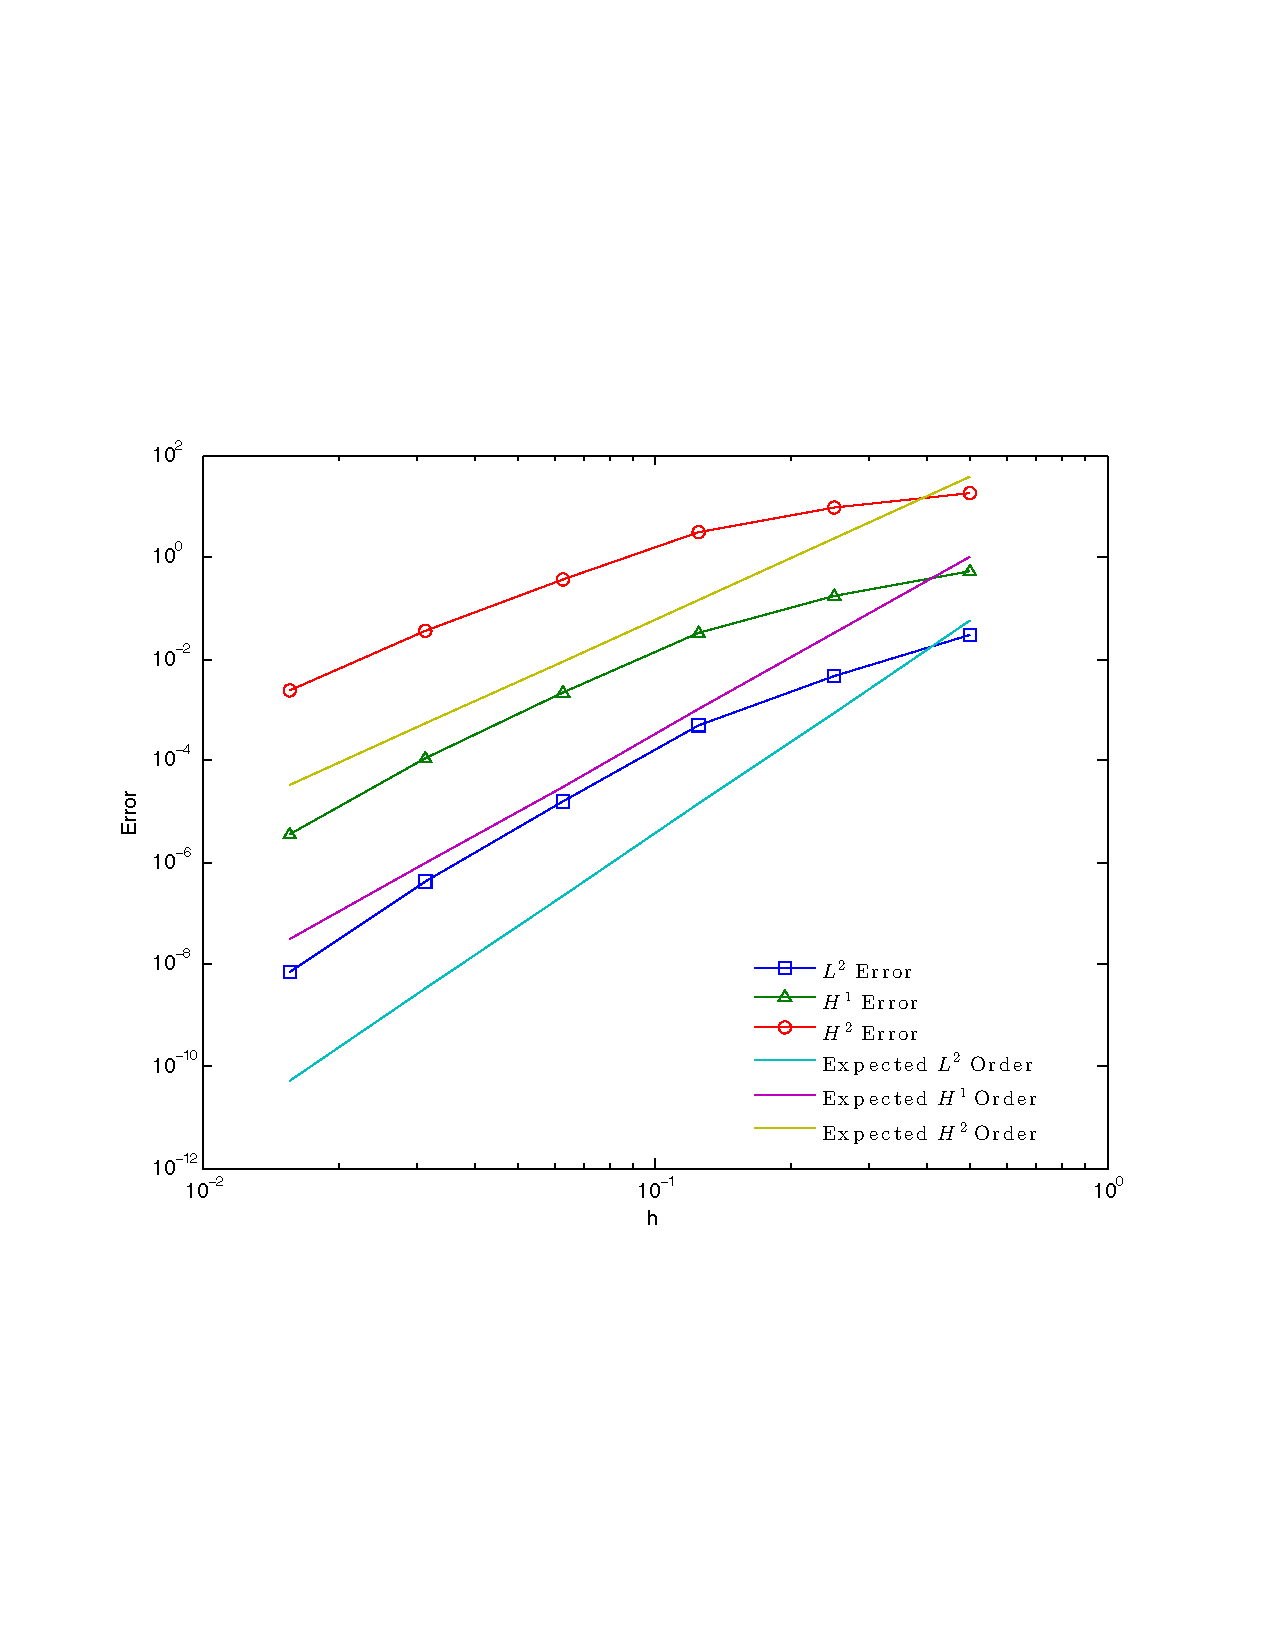
\includegraphics[scale=0.6]{Figures/expsinSpaceConvergence.pdf}
    \caption{Observed orders of convergence in space for Argyris applied to
      \eqref{eqn:QGE_psi} with the exact solution \eqref{eqn:Test2} using
      implicit Euler for the time discretization.}
  \label{fig:Test2Space}
  \end{center}
\end{figure}

%\subsection{North Atlantic}
%The North Atlantic Ocean is intensely studied and therefore makes a good test
%problem for evaluating the performance of our model \cite{Myers}. Hence, we have
%created a FE mesh of the North Atlantic which extend from $15^\circ N$ to $65^\circ
%N$ using GMSH \cite{GMSH}. The coastline data was obtain from GSHHS \cite{GSHHS}.
%The finite element spacing was specified to be {\color{red} $50km$}.  Major
%islands such as Cuba, Hispaniola Greenland, Great Britain, Ireland, Prince
%Edward Island, and Newfoundland were connected to the nearest continent and hard
%boundaries were created at the northern and southern most extents of the North
%Atlantic. Additionally, the Atlantic was closed off from the Mediterranean at
%the Straits of Gibraltar, the Mediterranean was closed off from the Black
%Sea at the entrance to the Sea of Marmara, and finally the Mediterranean was
%closed off from the Red Sea at the Suez Canal. The resultant FE mesh can be seen in
%\autoref{fig:AtlanticMesh}.
%
%\begin{figure}
%  \begin{center}
%    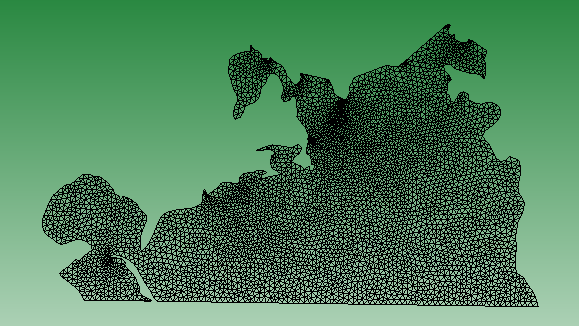
\includegraphics[scale=0.5]{NAMesh.png}
%    \caption{Mesh of the North Atlantic created using GMSH \cite{GMSH}.}
%    \label{fig:AtlanticMesh}
%  \end{center}
%\end{figure}
%
%The experiment used annual mean wind forcing obtained from Hellerman and
%Rosenstein (1983). We choose similar similar parameters as those used in
%\cite{delSastre04} and are summarized in \autoref{tab:AtlanticParameters}.
%
%\begin{table}
%  \begin{center}
%  \begin{tabular}{|l|l|}
%    \hline
%    $A$ & $2000m^2s^{-1}$\\
%    \hline
%    $\theta_0$ & $40^\circ$ \\
%    \hline
%    $\omega$ & $7.2526\times 10^{-5}s^{-1}$ \\
%    \hline
%    $H$ & $1000m$ \\
%    \hline
%    $L$ & $1000km$ \\
%    \hline
%    $r_e$ & $6378.1km$ \\
%    \hline
%    $\rho$ & $1027 \nicefrac{kg}{m^3}$ \\
%    \hline
%  \end{tabular}
%  \end{center}
%  \caption{Table of parameter values used for the simulations of the North
%    Atlantic. \cite{delSastre04}}
%  \label{tab:AtlanticParameters}
%\end{table}
%
%Using the relation
%\begin{equation}
%  \beta = \frac{2\omega}{r_e}\cos \theta_0
%  \label{eqn:Beta}
%\end{equation}
%and the parameters given in \autoref{tab:AtlanticParameters} we see that
%\begin{equation*}
%  \beta \approx 1.742\times 10^{-11}\, m^{-1}\,s^{-1}.
%\end{equation*}
%Using this approximation for $\beta$ and \eqref{eqn:velocity_scale} with
%{\color{red}$\tau_0 = 0.6\, dyne\, cm^{-2}$ \cite{Hellerman} gives the following
%approximation for the characteristic velocity
%\begin{equation*}
%%  \begin{split}
%%    U &= \frac{3.1415 \cdot 0.6 dyne\, cm^{-2}}{1027 \nicefrac{kg}{m^3} \cdot
%%      1000\, m \cdot 1.742 \times 10^{-11}\,m^{-1}\,s^{-1} \cdot 1000\, km} \\
%    U = 1.054\times 10^{-2} \nicefrac{m}{s}.
%%  \end{split}
%\end{equation*}
%Therefore, the Rossby number is
%\begin{equation*}
%%  Ro = \frac{1.054\times 10^{-2} \nicefrac{m}{s}}{1.742\times 10^{-11} m^{-1}
%%    s^{-1} (1000 km)^2}
%  Ro = 6.051\times 10^{-4}
%\end{equation*}
%and the Reynolds number is
%\begin{equation*}
%  Re = 5.27.
%\end{equation*}}
%
%From the length scale $L$ and the velocity scale $U$ we see that the time scale
%is approximately $T = 3\, years$. Thus, a nondimensional time interval of
%$[0,120]$, which was also used by Bermejo et al \cite{delSastre04}, corresponds
%to a total of $360$ years. We use the same dimensional time step used in
%\cite{delSastre04}, which was $\Delta t = 2\, hours$. This time step corresponds
%to nondimensional time step of $k = 7.6053 \times 10^{-5}$. {\color{red} This
%may be unrealistic.}
%
%\subsection{Mediterranean}
%We have created a FE mesh of the the Mediterranean Sea using GMSH \cite{GMSH}. The coastline data was obtain from GSHHS \cite{GSHHS}.
%The finite element spacing was specified to be {\color{red} $15km$}.  Major
%islands such as Corsica, Sardinia, and Sicily were connected to the nearest land
%mass. Additionally, the Atlantic was closed off from the Mediterranean at
%the Straits of Gibraltar, while the Gulf of Corinth was treated as land. The
%resultant FE mesh can be seen in \autoref{fig:AtlanticMesh}.
%
%\begin{figure}
%  \begin{center}
%    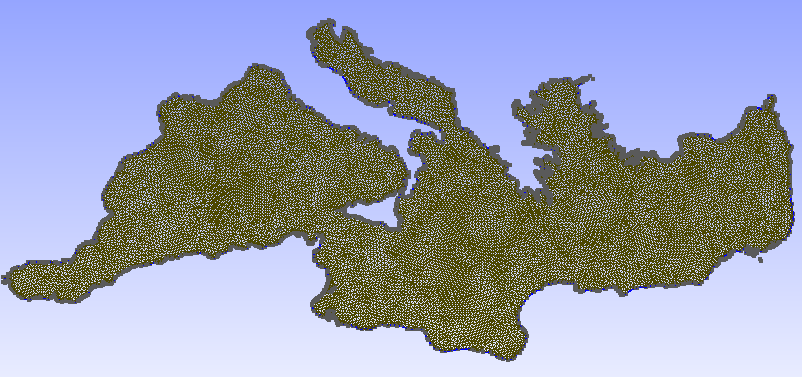
\includegraphics[scale=0.5]{MediterraneanMesh.png}
%    \caption{Mesh of the Mediterranean created using GMSH \cite{GMSH}.}
%    \label{fig:MedMesh}
%  \end{center}
%\end{figure}
%
